% MERGE - App-Model
%%%%%%%%%%%%%%%%%%%%%%%%%%%%%%%%%%%%%%%%%%%%%

%%%%%%%%%%%%%%%%%%%%%%%%%%%%%%%%%%%%%%%%%%%%%%%%%%%%%%%%%%%%%%%%%%%%%%%%%
% FR
\section{Visualisation}

% EN
%\section{Visualization}

% FR
Désormais, les services REST sont accessibles, nous savons ce qui est retournés et comment l'analyser avec l'application. Il nous reste plus qu'à faire tourner l'application afin de consulter les résultats.

Pour ce faire, il suffit d'ouvrir un navigateur web (Mozilla Firefox, Google Chrome, Safari...) et de renseigner l'URL du site ou bien d'ouvrir directement l'application depuis son mobile. On peut consulter le résultat :


% EN
% Now, the REST services are available, we know what is returned and how to analyze it in the application. It remains for us to run the application to see the results.

% To do this, simply open a web browser (Mozilla Firefox, Google Chrome, Safari ...) and write the site's URL. For the mobile, we can choose between the web browser or directly by the application. We can see the result : 

\begin{figure}[ht]
  \centering
  \begin{subfigure}[b]{0.6\textwidth}
    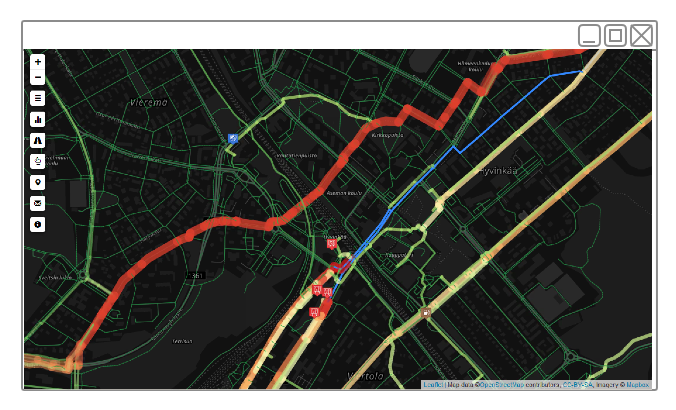
\includegraphics[width=\textwidth]
      {img/c03-merge/png/web-basemap-merge.png}
    \caption{Web}
  \end{subfigure}
  ~
  \begin{subfigure}[b]{0.2\textwidth}
    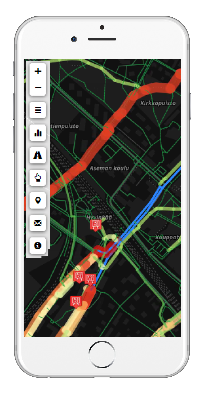
\includegraphics[width=\textwidth]
      {img/c03-merge/png/mobile-basemap-merge.png}
    \caption{Mobile}
  \end{subfigure}
  \caption{Combined display}
\end{figure}
